\documentclass[../../thesis.tex]{subfiles}
\graphicspath{{\subfix{diagrams/}}}

\begin{document}
The goal of the work is to explore if zk-rollups can be used to aggregate Uniswap trades in an effective manner. The prototype is able to aggregate trades for a single trading pair, Ether and an ERC-20 token of choice. The system consists of two main entites that are required for it to function. The first entity to look at, is the on-chain entity, we call zkSwap. zkSwap is a smart-contract deployed on the Ethereum blockchain and has three main jobs, processing deposits and withdraws, aswell as verifying batched trades. It holds users funds and exposes the on-chain functionality, namely deposits and withdrawls, to the user. 

The second entity to look at is the aggregator. The aggregator consists numerous systems, both off-chain and on-chain, and is mainly tasked with receiving trade orders, aggregating and executing them, and then verifying them with the zkSwap contract. The aggregator stores a merkle-tree of users balances and keeps it in sync by listening for event emitted by the zkSwap contract.

\begin{figure}[h]
    \centerline{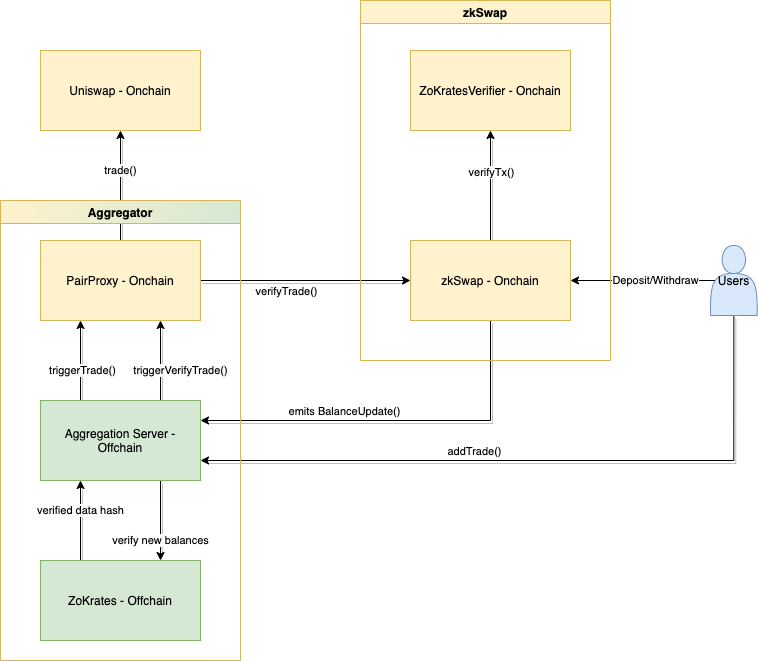
\includegraphics[totalheight=8cm]{diagrams/architecture.png}}
    \caption{High level architecture of the system}
    \label{fig:architecture}
\end{figure}


\subsection{zkSwap Contract}
The zkSwap contract, is the core entity the user interacts with. Its a smart-contract, that from the users perspective, is mainly used for depositing and withdrawing funds in out system. 

\subsubsection{Storing and Updating Balances} \label{balances}
Two main factors are dictating the way balances are stored in the system. It is important to understand the core technique used to store and update balances before we look at the different functions that trigger them. We want to make balance updates as cheap as possible, while not relying on any external data availability. Essentially, this means that we need to store the balances on-chain. Storing data on-chain is typically very expensive. It is important to make a distinction between storing data in a smart-contracts runtime and storing data in the event log. Both are on-chain, the event log is significantly cheaper though. While the event log is cheap to use and can be queried by any client, it is not accesible to a smart-contracts runtime. This solves the external data availablity problem. We can store data cheaply, without relying on other systems to stay online. A client can query the event log, gather the required data and pass it as parameters to the transaction. However, we now need a mechansism to ensure, the parameters passed are equal to the parameters found in the event log. 

We can achive this, be using a merkle tree \cite{szydlo2004merkle}. Merkle trees are a suitable data structure, as its root represents the entire tree state in a highly compressed form, while proving a leafs inclusion in the tree can be done with O(log n). This is ideal for our use-case. Every balance is stored as a leaf in a merkle tree, running in layer-2. The merkle tree is built and kept in sync by subscribing to the `BalanceUpdate' event emitted by our smart-contract. A client can query a balance from this tree, receiving the valid merkle path along with the data. Since the smart-contract stores the root of the balance merkle tree in its runtime, it can verify the correctness of the passed balance by hashing it along with the provided merkle path. If the resulting hash is equal to the stored root, the correctness of the balance is proven.\todo{Should I explain on what security assumptions this is based} Any changes to the balance data by the client will result in the hashes to mismatch, thereby invalidating the data. While the hashing of the balances and merkle path does create some fixed, overhead cost, the savings by using the event log far outstrip it. The hashing costs will be analysed in S. Results.

This fulfills the balance storage requirements, reducing costs, not relying on external data availabilty and ensuring the correctness of data. It must be noted, that this also causes the smart-contract to be the single source of 'truth'. Since all balances changes are committed by a new event being emitted and the root being updated, any balance updates must be done through the smart-contract. 

\subsubsection{Deposits and Withdraws}
When using the system, a user first has to deposit funds. Since the entire idea of zk-rollup is to move funds to layer-2, the deposit function can be seen as a bridge that connects the mainnet and layer-2. When a user makes a deposit, the funds are represented as a balance object in layer-2, which in turn give custody to these funds. When moving funds in layer-2, we don't actually move the funds residing in the smart-contract, but update the balance objects to represent the movement. Since a balance object gives a user custody of represented funds, it can always be redeemed, moving from layer-2 back to mainnet.  

As described in S. \ref{balances} balance updates are secured by merkle inclusion proofs in the smart-contract. When depositing the user needs to provide a valid merkle path to its balance object, and the balance object itself. The balance object consists of four fields that are needed to represent the balance: ethAmount, tokenAmount, nonce and userAddress. As a first step, the balance object is hashed with the sha256 algorithm, the result being the leaf in the merkle tree. The leaf is now hashed with the merkle path, according to the standart merkle root hashing algorithm. If the resulting hash equals the stored balance root in the contract, we can be assured that the balance object is correct. We now add the value of the transaction, which is the deposit amount sent with the transaction, to the ethAmount, increment the nonce and hash the new balance. Since the balance object has the same position in the tree, the same merkle path is also valid for the new balance. The new leaf is hashed with the merkle path, and the resulting hash is set as the new balance root. As a last step we emit the `BalanceUpdate' event, containing the new balance object, matching the balances with the newly set root. 

Withdraws largely follow the same logic, there are small differences though. As we're requesting funds, instead of sending them, we pass a withdrawAmount as an additional parameter to the function call. We then check if the withdrawAmount <= ethAmount to make sure the withdraw is covered by the users balance. The inclusion proofs are the same, we then subtract the withdrawAmount from the balance, and update the balance root. As a last step we emit the `BalanceUpdate' event with the new balance object, and send requested funds to the user as an on-chain transaction.

This however, is an incomplete explaination, as we're not checking if a user is permitted to deposit or withdraw funds. As balance objects are emitted as an event, anyone can access them and compute valid merkle paths for any balance. This would allow any user to withdraw any balance. To ensure a user is permitted to update a balance object, we need ensure the user controlls the private key belonging to the balance objects user address. Fortunetly we can ensure this by accessing the sender in transaction object. The Ethereum blockchain ensures a user is allowed to make a transaction by requiering the transaction to be signed with the private key of the senders address. If that signature is valid, it is proven that the user has access to the addresses private key and the transaction can be executed. Because of this, the transactions object sender can be trusted to be in controll of the corresponding private key. Instead of passing the users address as part of the balance object, the smart-contract uses the sender of the transaction object. This suffices as a security check.

It must also be noted, that ERC-20 deposits and withdraws behave a bit differently. As every ERC-20 token has its own smart-contract, representing a users balance as a mapping, we need to transfer the assets in that contract. This requires different functions to handle ERC-20 deposits and withdraws, however implementing this is trivial and not worth explaining in the context of this work. 

\begin{figure}[h]
    \centerline{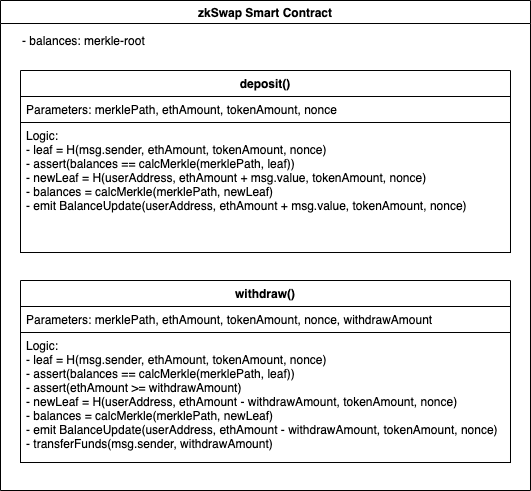
\includegraphics[totalheight=8cm]{diagrams/deposit_withdraw.png}}
    \caption{Pseudocode of the deposit and withdraw steps}
    \label{fig:dep_with}
\end{figure}

% This poses a problem, what use is a cheap data storage, if it can be queried from a client 


% The different functions that can be used to update balances will be described at a later point, 

% To achive this, we store balances in a merkle tree in layer-2, each balance stored as a seperate leaf. Merkle trees are a suitable data structure, as the root represents the entire tree state in a highly compressed form, while proving a leafs inclusion in the tree can be done with O(log n). This is ideal for our use-case. We can cheaply commit the merkle trees state to our smart-contract by storing the root, while verifying inclusion of a leaf is very efficient. The different functions that are can be used to update balances will be discussed at a later point, it is important to understand the core technique used for storing balances beforehand.
% The zkSync smart-contract is the only entity in the system that is able to update balances. Since we don't want to rely on external data availability, we need to store state on-chain, but as cheaply as possible. We can do this by emitting an event, thereby writing data to the event log. While the event log can't be accessed from a smart-contracts runtime, it is significantly cheaper then storing data in a smart-contracts storage. 
% a client can query the event log and pass the data as a parameter


% To deposit funds, a user need to provide a valid merkle path to its current balance and the current balance object. The user calls the deposit function, passing the merkle path and balance object as a parameter and adds the funds wishing to be deposited to the transaction. 

% First we check if the balance is included in the tree. To do this, we first hash the balance object with the sha256 algorithm. The balance object contains the following fields: ethBalance, tokenBalance, nonce and address. When hashing the balance object, we extract the users address from the transaction. This ensures that the user is in control of the addresses private key which suffices as security check. Since the contract stores the merkle root, we can now hash the path and balance, checking if we can recreate the root. If the roots match, the trader is permitted to update its balance in the tree. We now update the balance object by adding the deposited amount to the corresponding field, increment the nonce, hash the updated balance object, and rehash the entire tree with the the new balance object. The resulting merkle root is set in the contract, which commits the updated state. 

% However, we still need to store the balances somewhere. As we don't want to rely on external data availability, while keeping storage costs as low as possible, we emit the new balance as an event. Writing data to the event log is a lot cheaper, compared to storage as a variable in a smart-contract. While the event log can't be accessed from a smart-contracts runtime, a client can query the event log and pass the data as a parameter. As the merkle trees state is committed in the contract with the merkle root, correctness can always be proven. 

% Withdrawing funds follows the same logic as deposits. Instead adding funds to the withdraw function, the user passes the amount to withdraw as a parameter. The merkle tree is rehashed, checking if the root is correct, it is ensured the withdrawAmount <= balance, the balance and nonce are updated, creating the new root. We emit the new balance and send the funds to the user. 

% Deposits and withdraws are complete on-chain operations by design. All data needed to withdraw funds are public, except for the private key. This ensures funds can always be withdrawn, as long as the user controlls its private key.

% A trader can deposit funds, by providing a valid merkle path to its current balance as parameters to the zkSwap contract. 




% A trader looking to use the system first needs to deposit funds into the zkSync smart-contract.


% If successful, the deposited amount will be represented as a balance in layer-2. In layer-2, balance objects are stored in a merkle tree, while the root of that tree resides in the zkSync smart-contract. 

% and the amount represented as a balance in layer-2. 

% Since the goal is to store them in layer-2, while remaining free of any external data availability, a somewhat hybrid approach is needed. A trader always must be able to withdraw balance, no matter how many entities are offline. 

\subsection{zkSwap Contract}
Since we're looking to aggregate Uniswap trades, the obvious functionality required is for users deposit and withdraw funds, which will then in turn be used for trading. Users can deposit or withdraw funds by sending the corresponding transactions to the zkSwap contract, which will then


As mentioned before, the zkSwap contract is the only state-changing entity in this system. All state-changing operations are checked and then committed by this contract. This might be counter intuitive at first, as the goal is to move as much data as possible off-chain. It is important to remember though, that one main goal is not to rely on any external data availibility. This can only be achived by storing state on-chain, as compressed as possible. 

At the center of storing state is our system, is the root of the balance merkle tree, stored in the zkSwap contract. 


Since we're looking to aggregate Uniswap trades, the obvious functionality required is for users deposit and withdraw funds, which will then in turn be used for trading. As we're looking to move as much data as possible to layer-2. 
\end{document}